\chapter{Time-Dependent Shortest Path Calculation}\label{Chap:5}

\begin{defn}[\emph{FIFO Graph}]\label{Def:fifo_graph}
A time-dependent graph $G=(V,E)$ with a dynamic weight function $w : E,t \rightarrow \mathbb{R}$ is a FIFO graph \cite{TDS08} iff for every edge $(u, v) \in E$
\begin{equation}
\forall \Delta t \geq 0, \quad w(u, v, t_{0}) \leq \Delta t + w(u, v, t_{0} + \Delta t)
\end{equation}
\end{defn}

Chapter~\ref{Chap:4} discusses how to estimate the time-dependent travel cost of each signi\-ficant edge. Once the time-varying patterns of edge costs are determined, calculating a shortest path in a landmark graph is straightforward, provided the landmark graph is a FIFO graph\footnote{If the graph is not a FIFO graph, the problem is NP-hard if waiting is not allowed at any vertices} as defined in Definition~\ref{Def:fifo_graph}. 

An equivalent way of expressing FIFO property is that, if a person leaves vertex $u$ at time $t_{0}$, then any persons who leave vertex $u$ at a later time $t_{0} + \Delta t$ will not be able to reach vertex $v$ earlier than the first person. In practice, transport networks are said to have FIFO property \cite{TDR10}, therefore, a landmark graph can be considered as a FIFO graph. Then the Dijkstra's shortest path algorithm can be applied directly but with a modification that the edge costs are computed dynamically as the algorithm proceeds. Figure~\ref{Fig:dynamic_update} shows an example of dynamically updating edge costs. 

\begin{figure}[h!]
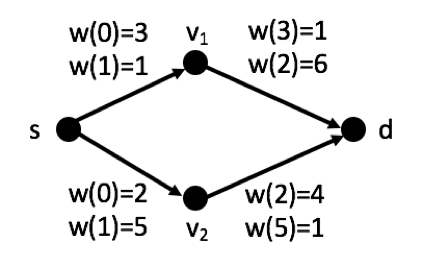
\includegraphics[scale=1]{shortest_path_demo}
\centering
\caption{An example of updating edge costs dynamically}\label{Fig:dynamic_update}
\end{figure}

If a taxi leaves $s$ at time $t = 0$, the edge $(s, v_{1})$ and $(s, v_{2})$ will have a time-dependent travel time of 3 and 2, respectively. If the taxi follows the current fastest edge $(s, v_{2})$, when it arrives at $v_{2}$ the time-dependent travel time of the edge $(v_{2}, d)$ at time $t = 2$ will be 4, giving a total travel time 6. But should the taxi follow the edge $(s, v_{1})$, the time-dependent travel time of the edge $(v_{1}, d)$ at $t = 3$ would be 1, giving a total travel time of 4. Therefore, path $s \leadsto v_{1} \leadsto d$ is the time-dependent shortest path. The same process applies when the taxi leaves $s$ at time $t = 1$, but the time-dependent shortest path will be path $s \leadsto v_{2} \leadsto d$. This example is also a FIFO graph: path $s \leadsto v_{1} \leadsto d$ would still be the shortest path, should another taxi \emph{wait} at $s$ until $t = 1$. Listing~\ref{List:code_dijkstra} gives the pseudocode for the modified Dijkstra's Algorithm. 

\begin{lstlisting}[language = Python, caption = {Pseudocode for Modified Dijkstra's Algorithm}, label = {List:code_dijkstra} ,frame=single, numbers=left,stepnumber=1, mathescape=true, escapeinside={(*}{*)}]
Input: a landmark graph $G=(V, E)$, a source $s$ (*and*) a destination $d$
Ouput: a predecessor graph $G_{p}=(V_{p}, E_{p})$
// EAT = Earliest Arrival Time
predecessor = dict{s : None}
pq = queue.PriorityQueue()
s.EAT = 0
pq.put(s)
for vertex in $G.V - \{s\}$:
    vertex.EAT = $\infty$
    pq.put(vertex)
while not pq.empty():
    hd = pq.get() // get the vertex at the queue head
    for v in hd.neighbours:
    	if hd.EAT + $w(hd, v, hd.EAT)$ < v.EAT:
	    v.EAT = hd.EAT + $w(hd, v, hd.EAT)$
	    predecessor[v] = hd
\end{lstlisting}

Upon termination of the algorithm in Listing~\ref{List:code_dijkstra}, a predecessor graph whose edges are \emph{reversed} shortest paths from $s$ to other vertices are constructed. Listing~\ref{List:code_printpath} provides a recursive method to print out the shortest path from $s$ to $d$. 

\begin{lstlisting}[language = Python, caption = {Pseudocode for Printing Shortest Paths}, label = {List:code_printpath} ,frame=single, numbers=left,stepnumber=1, mathescape=true, escapeinside={(*}{*)}]
Input: a predecessor graph $G_{p}=(V_{p}, E_{p})$ (*and*) a destination $d$
Ouput: a shortest path $s \leadsto d$

def print_path(predecessor, dst):
    pred = predecessor[dst]
    if pred is None:
    	print(dst.name)
    else:
    	print_path(predecessor, pred)
	print('$\rightarrow$' + dst.name)
	
print_path(predecessor, d)
\end{lstlisting}